\section{Advanced Users: How and When to create a RAVEN Template}
\label{sec:newTemplate}

One of the great strengths of the RAVEN input is its flexibility; an enormous number of different types of workflows can
%
be constructed with the components outlined in this manual. Sometimes, this flexibility is not required when standard or
%
predefined workflows need to be employed changing just few settings. For example, in classical uncertainty
%
quantification, sometimes only a few variables or the model needs to be changed, while the rest of the workflow stays
%
the same.
\\

As a tool to focus RAVEN on particular workflows, we introduce the RAVEN Templated Input Files. The intention of this
%
system is to allow a single user to develop a template RAVEN input file along with a template interface, thereby
%
simplifying inputs for any number of users that only need to make minor changes to the templated workflow in order to
%
perform their analysis.
\\

\nb A RAVEN Template is a wrapper for creating RAVEN input files; it is not part of the RAVEN core code and is usually s
%
specific to a particular application.

\subsection{When to use a RAVEN Template}
%
By design, a RAVEN Template simplifies the user experience at the cost of flexibility. The amount of streamlining is
%
adjustable and specific to each template. At one extreme, a Template takes no modifications at all and always produces
%
the same workflow; at the other extreme the Template duplicates entirely the RAVEN input syntax. Neither of those
%
options is desirable; Templates should find ground in-between.
\\

There are some times where using a RAVEN Template can be highly beneficial:
%
\begin{itemize}
  \item The workflow in question is highly complex, involving some advanced RAVEN usage to perform unorthodox calculations,
  %
  \item The workflow is mostly the same for each user, requiring only a small number of changes to use repeatedly.
\end{itemize}

There are some times when using a RAVEN Template is unlikely to be useful:
%
\begin{itemize}
  \item The workflow needs to be flexible enough to accommodate many unpredictable changes,
  %
  \item The workflow has few entries and can be changed manually quite easily.
\end{itemize}

\subsection{How to create a RAVEN Template}
%
A RAVEN Template consists of three main pieces: a Templated Workflow, a Template Class, and a Template Interface. The
%
Interface is the main driver, and uses an input file to inform the Template Class on how to modify the Templated
%
Workflow in order to create a new RAVEN input file.

\begin{figure}[h!]
 \centering
 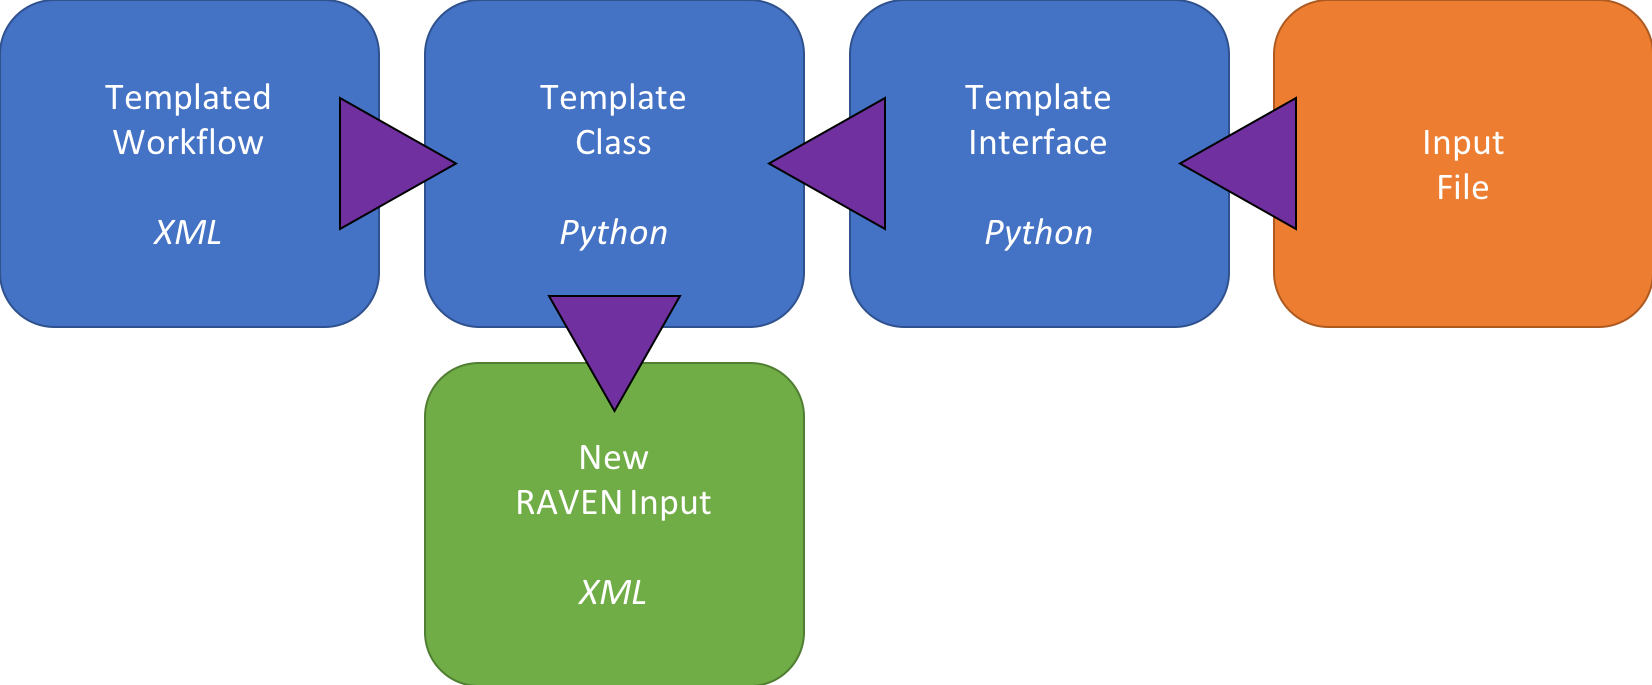
\includegraphics[width=\textwidth]{pics/TemplateWorkflow.png}
 \caption{Information Flow for RAVEN Templates}
 \label{fig:raven template workflow}
\end{figure}

Refer to Figure \ref{fig:raven template workflow}. Each box represents a file in a RAVEN template system. The three
%
boxes in blue (Templated Workflow, Template Class, and Template Interface) are developed collectively as the Template
%
by a designer familiar with RAVEN input files and Python. The development of this template only needs to occur once. The
%
orange box (Input File) is in a format determined by the Template Interface, and is the only portion of the Template
%
that a user will interact with repeatedly for any given workflow. The green box (New RAVEN Input) is the result of
%
reading a particular input file with the Template and is written by the Template. This new input can either be run
%
automatically with RAVEN or left to run at the user's convenience, based on what the Template Interface is designed to
%
do. Note that running RAVEN from within a python script on Windows within MinGW is particularly tricky.
\\

The three portions of the Template are discussed individually in the following sections.

\subsubsection{Templated Workflows}
%
A Templated Workflow begins with a traditional RAVEN input file that is run to do a particular analysis. It is highly
%
recommended that this workflow is run with RAVEN and the inputs and outputs are well understood before beginning
%
templating. Keep a copy of the original workflow before modifying the Templated Workflow.
\\

Next, consider the parts of the workflow that are common to anyone who will want to perform a similar analysis, and
%
which are specific to individual runs. For example, perhaps the \xmlNode{Sequence} and \xmlNode{Steps} are always the
%
same, but the \xmlNode{Model} and sampled \xmlNode{variable} nodes may change for each analysis. Note those parts of the
%
original workflow that need to be flexible, and remove them from the Templated Workflow. These will be filled in by the
%
Template Class for this workflow when the Template Interface is run.



\subsubsection{Template Class}
%
The Template Class is a bridge between the template designer and the Templated Workflow. The Template Class knows every
%
detail about the Templated Workflow and knows how to modify it to create a working RAVEN input.  It does so through a
%
set of standardized calls from the Template Interface.

A Template Base Class is provided in the RAVEN repository to be inherited by your new Template Class. It is located in
%
\begin{lstlisting}[language=bash]
 raven/framework/InputTemplates/TemplateBaseClass.py
\end{lstlisting}
%
We recommend you locate your new Template Class near your project where the workflows are run, and not in the RAVEN
%
repository.

There are several required methods in the API of the Template Base Class that are important.
%
\begin{lstlisting}[language=python]
 loadTemplate(self, filename, path)
\end{lstlisting}
%
The \texttt{loadTemplate} method is how the Template Class knows how to load the Template Workflow. The default
%
implementation in the Template Base Class is probably sufficient for most Template Classes, where given the filename and
%
path to the file, the template is loaded into \texttt{self.\_template}. Of course, this behavior can be modified however
%
suits a project by overloading this method in the Template Class.

\begin{lstlisting}[language=python]
 createWorkflow(self, **kwargs)
\end{lstlisting}
%
The \texttt{createWorkflow} method is the main method of the Template Class. The Template Interface calls this method
%
when it wants to use a series of modifications to write a new RAVEN input file. Note the Template Base Class
%
implementation of \texttt{createWorkflow} accepts arbitrary keyword arguments as \texttt{**kwargs}. This allows the
%
inheriting Template Class to define its own required arguments necessary to write a new input file. These may be lists,
%
dictionaries, or any other Python object. All of the necessary information for the Template Class to convert a Template
%
Workflow into a valid RAVEN input file should be passed through these arguments.
\\

The rest of \texttt{createWorkflow} is open to do any operations necessary to modify the XML in the Template Workflow
%
until it becomes a valid RAVEN input that performs the desired analysis. RAVEN offers a plethora of handy XML tools in
%
\texttt{raven/framework/xmlUtils}, which is imported in the base class and can be imported in your Template Class as
%
well. In addition, the Python standard library has an excellent \texttt{xml.etree.ElementTree} package for manipulating
%
XML.  Note that any \texttt{createWorkflow} should start by deepcopying the template XML, to assure a clean copy is
%
available each time it is called. The \texttt{createWorkflow} ends by returning the modified XML element.

\begin{lstlisting}[language=python]
 writeWorkflow(self, template, destination, run=False)
\end{lstlisting}
%
Once \texttt{createWorkflow} is called, the resulting XML element can be supplied to the \texttt{writeWorkflow} method,
%
which writes the XML to a file. The Template Base Class implementation will likely cover the needs of most Template
%
Classes, and shouldn't require significant modification. Note that an optional argument \texttt{run} instructs the
%
Template Class to attempt to run the workflow in RAVEN once it is written to file. Note this currently works on Mac
%
and Linux systems, but is not yet consistent on Windows.
\\

Other optional methods also exist in the Template Base Class and may be of use to individual templates.
%
\begin{lstlisting}[language=python]
 addNamingTemplates(cls, templates)
\end{lstlisting}
%
Note that the Template Base Class has a class-level dictionary member called \texttt{namingTemplates}. The intention of
%
this method is to store common ways to name items in the RAVEN input in a format method so that later they are always
%
consistent. To extend this method, call \texttt{BaseClass.addNamingTemplates} at the class level in the inheriting
%
Template Class.
\\

Finally, commonly-used shortcuts are included at the end of the Template Base Class to perform actions that are
%
repetitively used in modifying RAVEN inputs. We recommend you add your own to your Template Class to help keep
%
\texttt{createWorkflow} clean and easily maintainable.



\subsubsection{Template Interface}
%
The Template Interface is the code that actually gets called by users once the Template Class and Template Workflow are
%
complete. In its simplest form, the Template Interface is a Python script that reads the data needed for the
%
\texttt{createWorkflow} method and calls the methods on the Template Class in order:
%
\begin{enumerate}
  \item \texttt{loadTemplate}
  \item \texttt{createWorkflow}
  \item \texttt{writeWorkflow}
\end{enumerate}
%
Template Interfaces read a simplified input file so that users can provide their parameters for the Templated Workflow
%
in an easy manner. Whatever enables the use of the RAVEN workflow with minimal effort on the part of the users is ideal
%
for the Template Interface.





\subsection{Example}
%
For testing and as an example of implementation, a simple Template was created to perform basic uncertainty
%
quantification (UQ) analysis on external models. The example can be found in
%
\begin{lstlisting}[language=bash]
 raven/tests/framework/TemplateInputs
\end{lstlisting}
%
The following files are part of this template under the directory given above:
%
\begin{itemize}
  \item Templated Workflow: \texttt{TemplateInputs/UQTemplate/uq\_template.xml}
  %
  \item Template Class: \texttt{TemplateInputs/UQTemplate/UQTemplate.py}
  %
  \item Template Interface: \texttt{TemplateInputs/uq\_maker.py}
  %
  \item Input File: \texttt{TemplateInputs/UQTemplate/uq\_template\_input.i}
\end{itemize}
%
The original workflow from which the Templated Workflow was created involved a simple Monte Carlo sampling of an
%
external model and then postprocessing with BasicStatistics to find the mean, standard deviation, skewness, and kurtosis
%
of the results. The Template designer determined that this workflow could be used for many similar analyses with only
%
small changes, and decided to template it. The designer determined that things that could be changed include the model
%
sampled, the outputs of the model, the inputs to the model (with their distributions), and the number of Monte Carlo
%
samples to take. The designer also decided that each case should have its own WorkingDir to keep analyses separate. We
%
will consider the resulting Template files that the designer wrote one at a time in the following sections.



\subsubsection{Example Templated Workflow}
%
The file \texttt{uq\_template.xml} looks much like a typical RAVEN input file with some key pieces missing. The
%
\xmlNode{Sequence} shows that the two steps are \xmlString{sample} and \xmlString{stats}, which are for sampling a model
%
using Monte Carlo sampling and then performing some statistics on the results. Note however the missing contents in the
%
\xmlNode{WorkingDir}, the empty nodes in the \xmlNode{DataObjects}, the lack of any \xmlNode{Distributions}, and the
%
missing variable lists in the xmlNode{PostProcessor}. All the missing contents are filled in by the Template Class. For
%
the results of the filled-in workflow, see in
%
\begin{lstlisting}[language=bash]
 raven/tests/framework/TemplateInputs/gold/UQTemplate/new_uq.xml
\end{lstlisting}



\subsubsection{Example Template Class}
%
The file \texttt{UQTemplate.py} demonstrates inheritance of the Template Base Class and customization for the logic to
%
fill in the Templated Workflow.
\\

Note that the Template Class adds three formatted strings to the class-level name templates, one each for step names,
%
distributions, and metric variables. These are called later in the code to assure the naming conventions are always the
%
same. These formatted strings employ Python's inherent string formatting tools.
\\

The Template Base Class implementation of \texttt{loadWorfklow} does everything this Template needs to load the
%
Templated Workflow, so there is no need to modify it in the custom Template Class. Similarly, the \texttt{writeWorkflows}
%
does everything this Template needs to write a newly-created input, so there is no need to modify it in the custom
%
Template Class.  Since there was no need to overload the Template Base Class implementations of \texttt{loadWorfklow}
%
and \texttt{writeWorkflows}, the only main method changed in the Template Class is the essential \texttt{createWorkflow}
%
method. Note that we've added several keywords to the argument list:
%
\begin{lstlisting}[language=python]
  def createWorkflow(self, model=None, variables=None, samples=None, case=None, **kwargs):
\end{lstlisting}
%
In order to correctly modify the Templated Workflow, the Template Class needs to know about what model is being sampled,
%
the input variables to the model and how they're distributed, how many Monte Carlo samples to take, and the name of the
%
case being run. It requires all of these to be provided by the Template Interface in order to write a new RAVEN input.
%
In this case, the method arguments \texttt{model} and \texttt{variables} are dictionaries, while the \texttt{samples}
%
are an integer and the \texttt{case} is a string.
\\

Note that \texttt{UQTemplate.createWorkflow} calls the Template Base Class's implementation first in order to preserve
%
inheritance. Since the deepcopy happens in the base class, we don't perform it again in the custom Template Class.
\\

Throughout the remainder of the workflow creation, a series of XML manipulations are performed based on the inputs
%
provided from the Template Interface. For example, the module to load for the Model is changed, the working directory is
%
set, and the input and output variables are propagated throughout the input file. Note also that several input
%
construction shortcut methods have been added for this particular template to simplify maintenance of the template.


\subsubsection{Example Template Interface}
%
The file \texttt{uq\_maker.py} contains the basic logic needed to read a user input file, load the Template Class, and
%
generate new inputs. It follows the sequence of events outlined above, first instructing the Template Class to load the
%
template, then reading in the user input, then instructing the Template Class to create the workflow, then to write the
%
workflow.
\\

Beause the input needs for this Template are simple, we use Python's standard library \texttt{configparser} to read in
%
the user input file, \texttt{uq\_template\_input.i}. This simple input structure uses sections (model, variables, and
%
settings) with keyword and value pairs in each section. In order to change the RAVEN workflow created, the user only
%
needs to make changes to the existing input file and run the interface, then run RAVEN on the new input.
\\

Note that we chose to provide the information to the Template Class mostly through dictionaries, where the essential
%
pieces of information can be provided. In particular note that the variables provide only a mean and standard deviation;
%
one reduction in flexibility is that we assume the variables are normally distributed, disallowing other distributions.
\\

The Template can be run with Python from the command line:
%
\begin{lstlisting}[language=bash]
 > python uq_maker.py
 > cd UQTemplate
 > ~/projects/raven/raven_framework new_uq.xml
\end{lstlisting}
%
It reads in the user input, modifies the template, writes the new input file, and finally runs RAVEN. Note that, if
%
desired, the interface can be extended to perform additional operations after RAVEN has finished creating the workflow.
